%-----------------------------------------------------------------------------------------------
\makeatletter
\immediate\write18{datelog > \jobname.info} % site script for $(date '+%Y-%m-%d %Hh%Mm%Ss')
\makeatother
%-----------------------------------------------------------------------------------------------
%-----------------------------------------------------------------------------------------------
\usetheme{Copenhagen}
\usepackage{beamercolorthemeCNThermSci2}
\usefonttheme{serif}
%-----------------------------------------------------------------------------------------------

%-----------------------------------------------------------------------------------------------
%-----------------------------------------------------------------------------------------------
\usetheme{Copenhagen}
\usepackage{beamercolorthemeUTF2}
\usefonttheme{serif}
%-----------------------------------------------------------------------------------------------
\usepackage[utf8]{inputenc}
\usepackage[greek,french,english,brazil]{babel} % last becomes the active one
\usepackage{pslatex}
\usepackage{amssymb,amsmath}
\usepackage{soul}
\usepackage[squaren,Gray,cdot]{SIunits}
\usepackage[nice]{nicefrac}
\usepackage{tikz}
\usepackage{amscd}
\usepackage{stmaryrd}
\usepackage{scalerel}
\usepackage{xspace}
%-----------------------------------------------------------------------------------------------


%-----------------------------------------------------------------------------------------------
%-----------------------------------------------------------------------------------------------
% Mathematical
%-----------------------------------------------------------------------------------------------
\newcommand{\vet}[1]{\underline{{#1}}}
\newcommand{\mat}[1]{\underline{\underline{{#1}}}}
\newcommand{\cub}[1]{\underline{\underline{\underline{{#1}}}}}
\newcommand{\eqdef}{{\ensuremath\stackrel{\text{\tiny def}}{=}}}
%-----------------------------------------------------------------------------------------------
% Linguistic
%-----------------------------------------------------------------------------------------------
\newcommand{\GRtxt}[1]{\begin{otherlanguage}{greek}{{#1}}\end{otherlanguage}}
\newcommand{\FRtxt}[1]{\begin{otherlanguage}{french}{{#1}}\end{otherlanguage}}
%-----------------------------------------------------------------------------------------------
% Presentation
%-----------------------------------------------------------------------------------------------
\newcommand{\BkgImgH}[1]{% Places an image centered on the slide background filling the height
    \usebackgroundtemplate{\parbox{\paperwidth}{%
        \vspace*{1sp}\centering\includegraphics[height=\paperheight]{{#1}}
}}}
\newcommand{\BkgImgW}[1]{% Places an image centered on the slide background filling the width
    \usebackgroundtemplate{\parbox{\paperwidth}{%
        \vspace*{1sp}\centering\includegraphics[width=\paperwidth]{{#1}}
}}}
\newcommand{\ArtEndH}[3]{% Transitions to plain image (last) slide: #1:prefix #2,#3:extensions
    \BkgImgH{root/../art/#1.#2}
    \frame<handout:0>[plain]{%
        \transdissolve\vspace*{72mm}\color{white}\scriptsize\bf\input{root/../art/#1.#3}}
    \usebackgroundtemplate{\mbox{~}}
}
\newcommand{\ArtEndW}[3]{% Transitions to plain image (last) slide: #1:prefix #2,#3:extensions
    \BkgImgW{root/../art/#1.#2}
    \frame<handout:0>[plain]{%
        \transdissolve\vspace*{72mm}\color{white}\scriptsize\bf\input{root/../art/#1.#3}}
    \usebackgroundtemplate{\mbox{~}}
}
\newcommand{\ImgColW}[3]{% Inserts a full-width image in a column
    \includegraphics[width=\columnwidth]{root/../art/#1.#2}\\[-0.5\baselineskip]
    \parbox{\columnwidth}{\tiny\hfill\scalebox{0.85}{\input{root/../art/#1.#3}}}
}
\newcommand{\txtpic}[1]{%
    \fcolorbox{lightgray}{white!90!black}{{#1}} 
}
%-----------------------------------------------------------------------------------------------


%-----------------------------------------------------------------------------------------------
\title{C.02.01 -- Ciclo Otto Ar-Combustível de Tempo Finito de Combustão}
\subtitle{FTAF -- Finite Time Air-Fuel Otto Engine Model}
\author{Prof.~C.~Naaktgeboren, PhD}
\date{{\scriptsize\tt%
    
\includegraphics[height=6.0mm]{root/00-res/cc/by-nc-nd-88x31.pdf}\\[\smallskipamount]
    https://github.com/CNThermSci/ApplThermSci\\
    Compiled on \input{\jobname.info}
}}
%-----------------------------------------------------------------------------------------------
\begin{document}
%-----------------------------------------------------------------------------------------------
\logo{%
    \parbox{158mm}{% There's a 1mm gap on each side of the 160mm x 90mm slide logo line
        \mode<beamer>{
            
\includegraphics[height=6.0mm]{root/00-res/UTFPR/UTFPR-logo-D.pdf}\hfill%
            
\includegraphics[height=9.0mm]{root/00-res/logo/CNThermSci-logo-A.pdf}%
        }
        \mode<handout>{
            
\includegraphics[height=6.0mm]{root/00-res/UTFPR/UTFPR-logo-W.pdf}\hfill%
            
\includegraphics[height=9.0mm]{root/00-res/logo/CNThermSci-logo-W.pdf}%
        }
    }
} % The (delineated, alpha), or washed-out logos
%-----------------------------------------------------------------------------------------------
\frame{\titlepage}
%-----------------------------------------------------------------------------------------------

%------------------------------------------------------------------------------------------------
\section{Apresentação do FTAF}
%-----------------------------------------------------------------------------------------------

%------------------------------------------------------------------------------------------------
\subsection{Como Extensão do FTAH}
%-----------------------------------------------------------------------------------------------

    % !j 96 -i8
    %-------------------------------------------------------------------------------------------
    \begin{frame}{Ciclo Otto ar-combustível de tempo finito---FTAF}\vspace*{-2em}
        \begin{itemize}
            \item<1->  Modelo do livro-texto (tópicos de leitura) adiciona \alert{combustão} ao
                \alert{Ciclo Otto ideal};
            \begin{itemize}
                \item<2->  Permite variação de \alert{combustíveis};
                \item<3->  Porém, desde que sejam \alert{carbonados}: norm.~em $C$;
                    \alert{excluindo \ce{H2}} e \alert{\ce{H4N2}} puros, p.~ex.;
                \item<3->  Ênfase nas \alert{propriedades} $\bar{c}_{p,v}(T)$, $k(T)$,
                    $\bar{u}(T)$, etc.~das misturas;
                \item<4->  Incorpora \alert{combustão} e \alert{equilíbrio químico};
                \item<5->  \alert{Não emprega} o calor liberado na \alert{combustão}!
            \end{itemize}
            \item<6->  Modelo \alert{ar-combustível de tempo finito, FTAF}:
            \begin{itemize}
                \item<7->  Adiciona \alert{combustão}, mantendo as demais características do
                    \alert{FTHA};
                \item<8->  Obtém tanto as \alert{propriedades} quanto o \alert{calor liberado}
                    pelas \alert{reações}!
                \item<9->  \alert{Permite} modelar combustão de \alert{HC's}, \alert{\ce{H2}} e
                    \alert{\ce{H4N2}}; tanto \alert{puros} quanto suas \alert{misturas}!
                \item<10-> Desenvolvido em um \alert{TCC} defendido em \alert{2018} (citação nos
                    tópicos de leitura);
                \item<11-> \alert{Não} modela a cinética química: tempos de combustão permanecem
                    dados de \alert{entrada}.
            \end{itemize}
        \end{itemize}
    \end{frame}
    %-------------------------------------------------------------------------------------------

    % !j 96 -i8
    %-------------------------------------------------------------------------------------------
    \begin{frame}{Ciclo Otto ar-combustível de tempo finito---FTAF}\vspace*{-2em}
        \begin{itemize}
            \item<1->  Modela combustão de forma \alert{não instantânea}:
            \begin{itemize}
                \item<2->  Interações \alert{simultâneas} de \alert{liberação de energia
                    interna} e \alert{trabalho};
                \item<3->  Tempos de motor \alert{discretizados} em \alert{sub-processos};
                \item<4->  Elemento computacional: sub-processo \alert{localmente politrópico}
                    em base \alert{extensiva};
                \item<5->  \alert{Remoção} de calor permanece \alert{isocórica} (instantânea);
                \item<6->  Requer modelos de mistura e reações \alert{não instantâneos}!
            \end{itemize}
            \item<7->  Não mais um modelo \alert{padrão a ar}:
            \item<8->  Não mais um modelo de \alert{substância pura}:
            \begin{itemize}
                \item<9->  Inclui \alert{combustão e equilíbrio químico};
                \item<10-> Requer modelagem termodinâmica de \alert{misturas reativas}.
            \end{itemize}
        \end{itemize}
    \end{frame}
    %-------------------------------------------------------------------------------------------

    % !j 96 -i8
    %-------------------------------------------------------------------------------------------
    \begin{frame}{Ciclo Otto ar-combustível de tempo finito---FTAF}\vspace*{-2em}
        \begin{itemize}
            \item<1->  Inclui todos os parâmetros do \alert{FTHA}:
            \begin{itemize}
                \item<2->  Todos os do \alert{ciclo Otto ideal}, mais
                \item<3->  Todos os parâmetros \alert{construtivos} do \alert{motor}, mais
                \item<4->  Todos os parâmetros \alert{operacionais} do \alert{motor};
            \end{itemize}
            \item<5->  Inclui parâmetros da \alert{mistura ar-combustível}:
            \begin{itemize}
                \item<6->  \alert{Proporções} dos gases do \alert{ar};
                \item<7->  \alert{Composições e proporções} do \alert{combustíveis};
                \item<8->  \alert{Proporções} da mistura \alert{ar-combustível} em relação à
                    \alert{estequiometria}.
            \end{itemize}
            \item<9->  \alert{Balanço de Energia} melhorado:
            \begin{itemize}
                \item<10-> \alert{Liberação de energia interna} pelas reações \alert{explícita};
                \item<11-> Com separação conceitual das \alert{transferências de calor}.
            \end{itemize}
        \end{itemize}
    \end{frame}
    %-------------------------------------------------------------------------------------------

%-----------------------------------------------------------------------------------------------
\section{Extensões FTAF}
%-----------------------------------------------------------------------------------------------

%------------------------------------------------------------------------------------------------
\subsection{Fração Cumulativa $y(\alpha)$}
%-----------------------------------------------------------------------------------------------

    % !j 96 -i8
    %-------------------------------------------------------------------------------------------
    \begin{frame}{Modelo de Evolução de Reação:}\vspace*{-2em}
        \begin{columns}
        \column{0.50\textwidth}
        \begin{itemize}
            \item<1->  \alert{Reações} evoluem com \alert{$y(\alpha)$}:
        \end{itemize}
        \vspace*{-1.0ex}\begin{align}
            \uncover<2->{
            \alert{y(\alpha)}   &\alert{=
            \begin{cases}
                0           & \mbox{para }\alpha < \theta,\\
                g(\alpha)   & \mbox{para }\theta \leqslant \alpha \leqslant \theta+\delta,\\
                1           & \mbox{para }\alpha > \theta+\delta.
            \end{cases}}\nonumber
            }
        \end{align}
        \vspace*{-3.0ex}\begin{itemize}
            \item<3-> \alert{$g(\alpha)$} modela o \alert{histórico} da reação química:
                \\[\smallskipamount]
            \begin{itemize}
                \item<4-> \alert{$g(\theta) = 0$} e \alert{$g(\theta+\delta) = 1$};
                    \\[\smallskipamount]
                \item<5-> \alert{Função} $g(\alpha)$ deve ser \alert{monotônica};
                    \\[\smallskipamount]
                \item<6-> $g(\alpha)$ pode basear-se em \alert{experimentos};
                    \\[\smallskipamount]
                \item<7-> Lit.:~\alert{$g(\alpha) = \frac{1}{2}-\frac{1}{2} \cos \bigl(
                    \frac{\pi}{\delta} (\alpha - \theta) \bigr)$}.
            \end{itemize}
        \end{itemize}
        \column{0.50\textwidth}
        \begin{center}
            \uncover<2->{\vspace*{-5mm}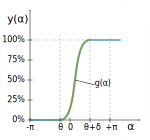
\includegraphics[height=70.0mm]{fig/FTAFTiming01.pdf}}
        \end{center}
        \end{columns}
    \end{frame}
    %-------------------------------------------------------------------------------------------

%------------------------------------------------------------------------------------------------
\subsection{Balanço de Energia e Estratégia de Solução}
%-----------------------------------------------------------------------------------------------

    % !j 96 -i8
    %-------------------------------------------------------------------------------------------
    \begin{frame}{Equações Termodinâmicas}\vspace*{-2em}
        \uncover<1->{
            Balanço de energia do $i$-ésimo (sub-)processo politrópico
            \alert{$P_iV_i^{\mathsf{n}_i} = P_{i+1}V_{i+1}^{\mathsf{n}_i}$}:
        }
        \begin{align*}
            \uncover<2->{
                Q_i - W_i
                    &= U_{m,i+1} - U_{m,i},
            }
            \uncover<3->{
                \quad\rightharpoondown\\[\medskipamount]
                Q_i + (U^0_{f,m,i} - U^0_{f,m,i+1}) - W_i
                    &= U^0_{m,i+1} - U^0_{m,i},
            }
            \uncover<4->{
                \quad\rightharpoondown\\[\medskipamount]
                \alert{U^0_{m,i+1}}
                    &\alert{= U^0_{m,i} + Q_i + \Delta{U_{reac,i}} - W_i},\qquad\mbox{com}
            }
            \uncover<5->{
                \\[\medskipamount]
                \alert{\Delta{U_{reac,i}}}
                    &\equiv U^0_{f,m,i} - U^0_{f,m,i+1}
                    \qquad\rightharpoondown \\[\medskipamount]
                    &\alert{= H^0_{f,m,i} - n_{m,i}\bar{R}T_0
                    - H^0_{f,m,i+1} + n_{m,i+1}\bar{R}T_0}.
            }
        \end{align*}
    \end{frame}
    %-------------------------------------------------------------------------------------------

    % !j 96 -i8
    %-------------------------------------------------------------------------------------------
    \begin{frame}{Equações Termodinâmicas}\vspace*{-2em}
        \begin{align*}
            \uncover<1->{
                \alert{Q_i}
                    &\alert{= \unit{0}{\kilo\joule}},
                    \qquad\mbox{ignorando transferência de calor com cabeçote, bloco, etc.}
            }
            \uncover<2->{
                \\[\medskipamount]
                \alert{W_i}
                    &\alert{= \begin{cases}
                        \dfrac{P_iV_i}{1-\mathsf{n}_i}\left[
                            1-\left(
                                \dfrac{V_i}{V_{i+1}}
                            \right)^{\mathsf{n}_i-1}
                        \right],
                        \quad & \mbox{para }\mathsf{n}_i \neq 1,
                        \\[\bigskipamount]
                        P_iV_i\ln\dfrac{V_i}{V_{i+1}},
                        & \mbox{para }\mathsf{n}_i = 1,
                        \\[\medskipamount]
                        \unit{0}{\kilo\joule},
                        & \mbox{para }V_i \approx V_{i+1}
                        \quad\rightharpoondown\quad
                        |V_i - V_{i+1}| \leqslant \epsilon_V.
                \end{cases}}
            }
        \end{align*}
    \end{frame}
    %-------------------------------------------------------------------------------------------



%------------------------------------------------------------------------------------------------
\subsection{Composição Instantânea do Sistema}
%-----------------------------------------------------------------------------------------------

    % !j 96 -i8
    %-------------------------------------------------------------------------------------------
    \begin{frame}{Mistura Ativa: Composição Instantânea}\vspace*{-2em}
        \uncover<1->{
            A composição \alert{instantânea} do sistema, que contém o \alert{fluido ativo}, é:
        }
        \begin{align*}
            \uncover<2->{
                \MXSYSi
                    &= (1 - y_i)\,\MXREA + y_i\,\MXPRO,
                    \qquad\rightharpoondown
            }
            \uncover<3->{
                \\[\medskipamount]
                \alert{\MXSYSi}
                    &\alert{= (1 - y_i)(1 - \zeta)\,\MXAFU}
                    \alert{+ [(1 - y_i)\zeta + y_i]\,\MXPRO},
            }
        \end{align*}
        \uncover<4->{
            com:
        }
        \begin{align*}
            \uncover<5->{
                \alert{\MXAFU}
                    &= \alert{\NF}\,\mbox{\ce{C\NC H\NH O\NO N\NN}}
                    \,+\alert{\NA}\left(
                            \alert{\frac{1}{1+\psi}}\mbox{\ce{O2}} +
                            \alert{\frac{\psi}{1+\psi}}\mbox{\ce{N2}}
                        \right)
                \qquad\mbox{e}
            }
            \uncover<6->{
                \\[\medskipamount]
                \alert{\MXPRO}
                    &=  \alert{\NCOO}\mbox{\ce{CO2}}
                    +   \alert{\NHHO}\mbox{\ce{H2O}}
                    +   \alert{\NCO}\mbox{\ce{CO}}
                    +   \alert{\NHH}\mbox{\ce{H2}}
                    +   \alert{\NOO}\mbox{\ce{O2}}
                    +   \alert{\NNN}\mbox{\ce{N2}}.
            }
        \end{align*}
    \end{frame}
    %-------------------------------------------------------------------------------------------

%-----------------------------------------------------------------------------------------------
\section{Tópicos de Leitura}
%-----------------------------------------------------------------------------------------------

    %------------------------------------------------------------------------------------------
    \begin{frame}[allowframebreaks]{Tópicos de Leitura}
        \begin{thebibliography}{Brunetti, F., 2012}
            \bibitem[Brunetti, F., 2012]{2012-BrunettiF-Blucher}
                Brunetti, F.
                \newblock{%
                    {\em Motores de combustão interna\/}.
                    \alert{Capítulos 1 e 2.}
                }
                \newblock{\footnotesize Blücher. São Paulo. ISBN 978-85-2120-708-5.}
            \bibitem[Silva, R.~K.~de O., 2018]{2018-SilvaRKO-UTFPR}
                Silva, R.~K.~de O.
                \newblock{%
                    {\em Modelo ar-combustível de tempo finito de adição de calor de motores
                    {O}tto\/}.
                }
                \newblock{\alert{Repositório Roca UTFPR.}}
                \newblock{\footnotesize repositorio.roca.utfpr.edu.br/jspui/handle/1/8786.}
        \end{thebibliography}
    \end{frame}
    %------------------------------------------------------------------------------------------

    % Finishes with stunning image, with credit
    \ArtEndW{pexels-kaboompics-com-5969}{jpg}{txt}

%-----------------------------------------------------------------------------------------------
\end{document}
%-----------------------------------------------------------------------------------------------

